\chapter{Demo -- Avances de Implementación}\label{chapter07}

A continuación se presentan capturas del sistema en funcionamiento (agosto de 2026), correspondientes al avance de implementación de este hito del 75\%: el pipeline de captura y su monitoreo, la base de datos histórica, la API REST y el dashboard con el ranking por score de tendencia. El sistema se encuentra publicado y accesible en producción, con captura de datos automatizada ejecutándose de manera autónoma varias veces por día. La interfaz web se divide en dos vistas: un panel para clientes (\texttt{/dashboard}), con el ranking de productos y la evolución del score en el tiempo, y un panel técnico interno (\texttt{/admin}) con el monitoreo de endpoints y los registros de minería, que se documenta a continuación como evidencia de RNF01.

\begin{figure}[ht]
	\centering
	
\includegraphics[width=0.75\textwidth]{./images/demo/demo_dashboard.png}
	\caption{Panel técnico interno del sistema en funcionamiento (agosto 2026).}
	\label{fig:demo-dashboard}
\end{figure}

\begin{figure}[ht]
	\centering
	
\includegraphics[width=0.9\textwidth]{./images/demo/demo_dashboard_apis.png}
	\caption{Panel de disponibilidad de endpoints (EndpointHealthLog): monitoreo registrado en cada sesión de minería.}
	\label{fig:demo-apis}
\end{figure}

\begin{figure}[ht]
	\centering
	
\includegraphics[width=0.85\textwidth]{./images/demo/demo_dashboard_score.png}
	\caption{Panel de clientes: ranking de productos por score de tendencia (RF02), con filtros por categoría y exportación CSV (RF03/RF06).}
	\label{fig:demo-score}
\end{figure}

\begin{figure}[ht]
	\centering
	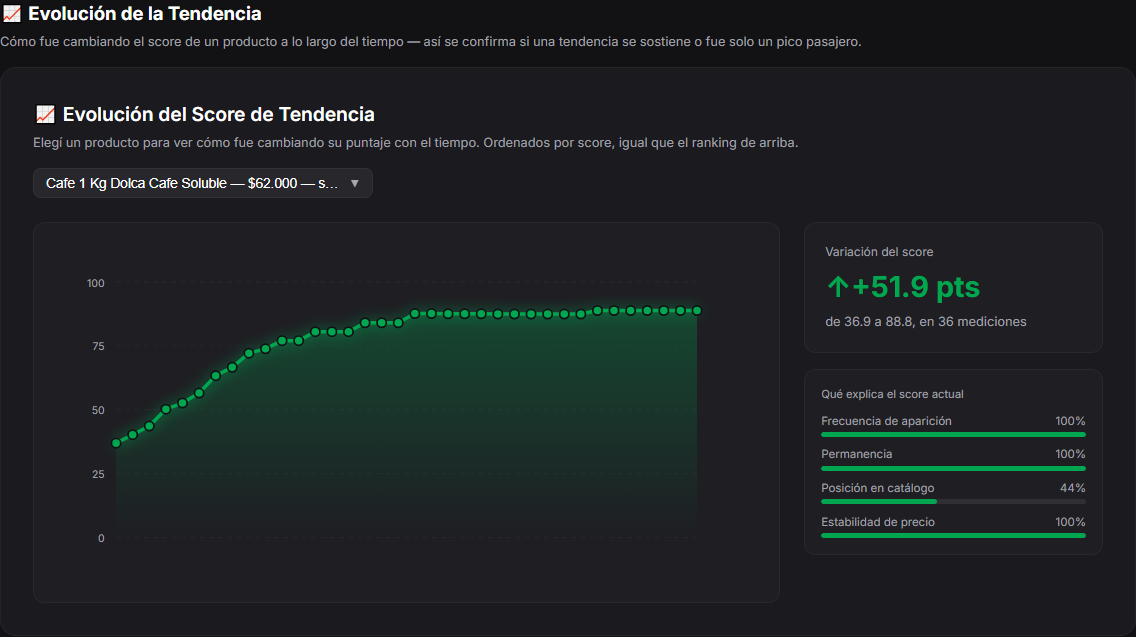
\includegraphics[width=0.85\textwidth]{./images/demo/demo_dashboard_evolucion.png}
	\caption{Panel de clientes: evolución del score de tendencia de un producto en el tiempo, con el desglose de sus componentes (RF02, RF05).}
	\label{fig:demo-evolucion}
\end{figure}

\section{Evidencia cuantitativa del sistema en producción}\label{sec:evidencia-cuantitativa}

Más allá de la afirmación de que el sistema está desplegado y capturando datos, esta sección documenta con números concretos, medidos directamente sobre la base de datos y los endpoints en producción, cómo se comporta el prototipo actual. Los volúmenes de datos se remidieron el 23/09/2026 para reflejar el crecimiento del histórico desde la primera medición (10/08/2026); los tiempos de respuesta mantienen la fecha de su propia medición, indicada en cada fila.

\begin{table}[H]
	\centering
	\small
	\caption{Métricas del sistema en producción (volúmenes de datos medidos el 23/09/2026)}
	\label{tab:evidencia}
	\begin{tabularx}{\textwidth}{@{}>{\raggedright\arraybackslash}p{5.2cm} X@{}}
		\toprule
		\textbf{Indicador} & \textbf{Valor medido} \\
		\midrule
		Rango temporal del histórico & 14/07/2026 -- 23/09/2026 (71 días de operación continua) \\
		Productos monitoreados & 274 \\
		Categorías monitoreadas & 6 (Computación, Celulares, Electrónica, Ropa y Accesorios, Alimentos y Bebidas, Limpieza del Hogar) \\
		Apariciones registradas (\texttt{TrendSnapshot}) & 5717 \\
		Registros de precio (\texttt{PriceHistory}) & 5807 \\
		Scores de tendencia calculados (\texttt{TrendScore}) & 11539 \\
		Registros de monitoreo de endpoints (\texttt{EndpointHealthLog}) & 1899 \\
		Sesiones de minería estimadas & $\sim$203 (agrupando snapshots por cortes de inactividad $>$40 min), $\sim$28,2 apariciones registradas por sesión en promedio \\
		Frecuencia de captura configurada & 3 corridas diarias (cron programado, ver Sección~\ref{sec:evolucion-tecnica}) \\
		Tiempo de respuesta -- \texttt{/api/health}, \texttt{/api/status} & 0,5 -- 2,1\,s (medido, 3 muestras c/u) \\
		Tiempo de respuesta -- \texttt{/dashboard} (panel de clientes) & 0,5 -- 1,1\,s en caliente (medido, 5 muestras el 15/08/2026, tras separar el panel de clientes del panel técnico) \\
		Tiempo de respuesta -- \texttt{/admin} (panel técnico) & 1,9 -- 4,0\,s (medido, 3 muestras el 15/08/2026) \\
		Tiempo de respuesta -- \texttt{/api/trend-scores} & 1,7 -- 2,9\,s en caliente (medido, 5 muestras el 21/09/2026, tras la corrección de RNF02 -- ver Sección~\ref{sec:pruebas}) \\
		\bottomrule
	\end{tabularx}
\end{table}

Un ejemplo real de exportación CSV (RF06) generado desde el dashboard el mismo día incluye columnas \texttt{producto, categoria, precio, moneda, variacion\_pct, score, periodo, calculado, link}, con una fila por cada producto del ranking filtrado en pantalla al momento de la exportación (ver Figura~\ref{fig:demo-score}).

Un hallazgo temprano de esta medición (10/08/2026) fue que \texttt{/api/trend-scores} -- el endpoint que alimenta el ranking principal -- no cumplía el objetivo de RNF02 (respuesta en menos de 3 segundos): la consulta traía los 3911 scores históricos con sus relaciones completas en cada solicitud, en lugar de traer solamente las últimas mediciones vigentes por producto. La corrección aplicada y su verificación posterior en producción se documentan en la Sección~\ref{sec:pruebas}.

\section{Pruebas funcionales y resultados}\label{sec:pruebas}

Sobre el sistema en producción se aplicaron dos técnicas de prueba distintas: pruebas de rendimiento sobre los requerimientos no funcionales, y una prueba de usabilidad embebida en una entrevista con un usuario real.

\subsection*{Pruebas de rendimiento (RNF02)}

La medición del 10/08/2026 (Tabla~\ref{tab:evidencia}) mostró que \texttt{/api/trend-scores} respondía en 6,3--7,6\,s, por encima del objetivo de 3\,s de RNF02. La causa identificada fue que la consulta traía el historial completo de \texttt{TrendScore} (más de 7700 filas a esa fecha) con el historial de precios de cada producto anidado, cuando el dashboard solo necesita las últimas 2 mediciones por producto para calcular la variación mostrada en pantalla. La corrección, aplicada acotando la consulta a esas últimas 2 mediciones, se verificó nuevamente en producción el 21/09/2026 con 5 muestras adicionales: el tiempo de respuesta bajó a 1,7--2,9\,s en caliente, dentro del objetivo. RNF02 pasa así de \emph{Parcial} a \emph{Implementado} en la matriz de trazabilidad (Sección~\ref{sec:trazabilidad}).

\subsection*{Prueba de usabilidad}

La Entrevista 2 (Anexo D, Sección~\ref{chapter06}) incluyó una instancia de prueba de usabilidad: se mostró el dashboard en funcionamiento a un vendedor real (Lucas) y se le pidió que interpretara la pantalla sin explicación previa (pregunta 3, ``¿Qué entendés que muestra esta pantalla?''). El entrevistado identificó correctamente el propósito del ranking y del score sin asistencia, lo que valida que la interfaz comunica su función principal sin necesidad de instrucciones adicionales.

Esa misma instancia motivó una decisión de diseño a partir de sus resultados: la pregunta sobre qué le faltaba a la herramienta (pregunta 8) y la objeción de que el score funcionaba como una ``caja negra'' (pregunta 10) llevaron a que el desglose de sus cuatro componentes -- frecuencia, permanencia, ranking, estabilidad -- se muestre explícitamente en el dashboard en lugar de solo el puntaje final, decisión ya documentada en la Sección~\ref{sec:score-formal}.
